\chapter{La zone des liens}

La zone des liens est une zone contenant les diff�rents liens
principaux de l'application. Cette zone est statique et diff�re selon
l'utilisateur. 
Par exemple, on peut voir apparaitre le lien {\it se d�connecter} pour
l'enseignant et l'administrateur qui
n'aurait aucune utilit� pour le consultant.\\
De m�me, quant � la recherche, selon l'utilisateur, le(s) type(s) de
donn�e(e) pouvant �tre recharch�(s) sera(ont)
diff�rent(s). L'utilisateur pourra effectuer une recherche multiple,
c'est-�-dire par exemple, les TD et projets simultan�ments.\\
Pour le consultant, appraissent des liens de th�me tel que {\it Java}
qui repr�sente en fait une recherche compl�te avec comme mots cl�s Java.
\begin{flushleft}
\scalebox{0.6}{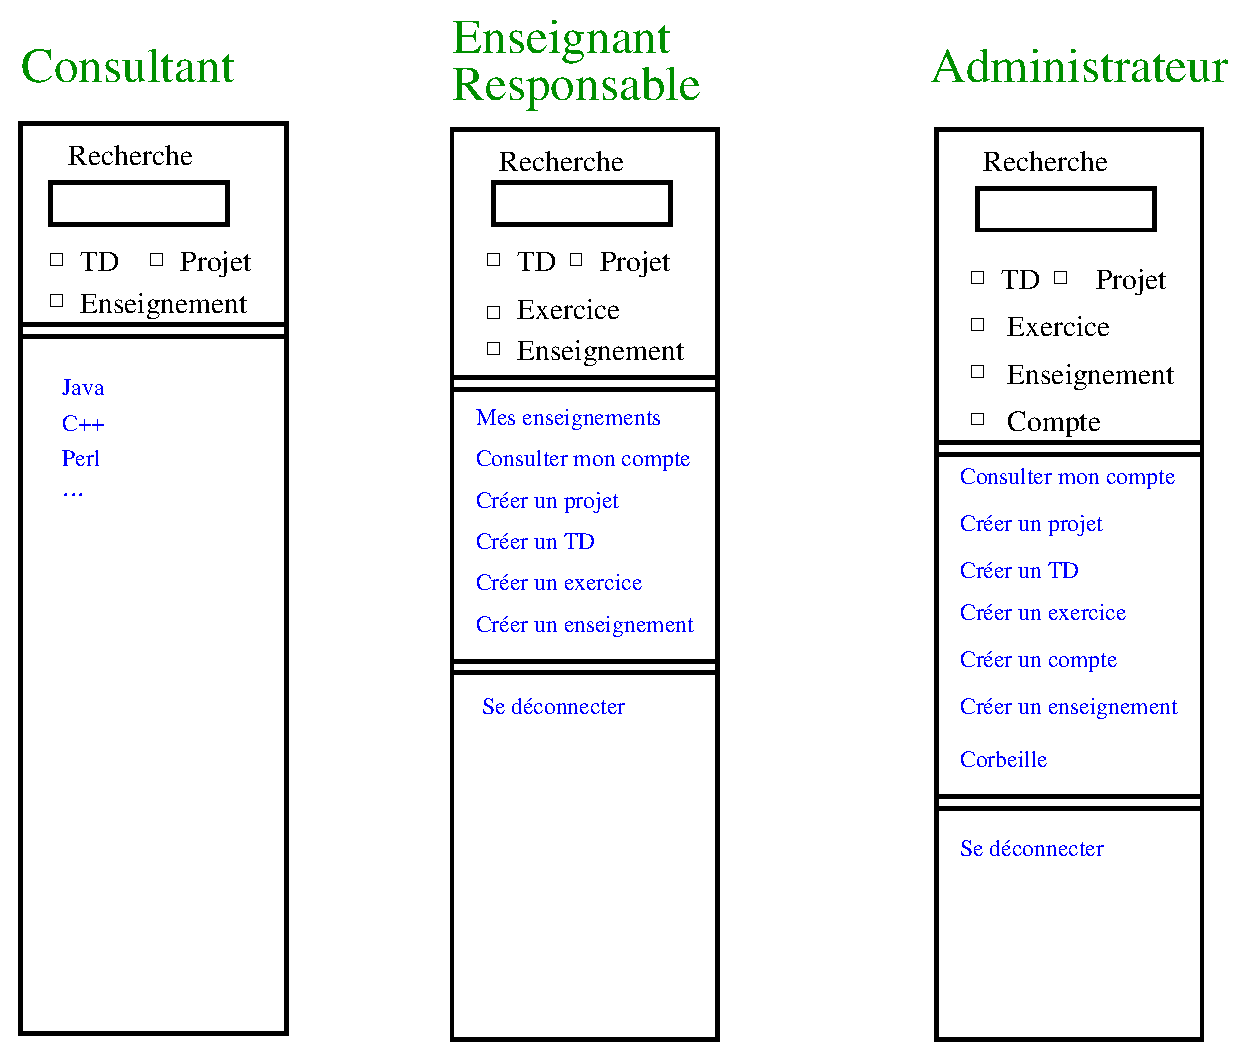
\includegraphics{../eps/Liens.eps}}\\
\end{flushleft}


